\section{Technical standards}
\label{sect:standards}
In this section we define explicitly the technical data exchange format for the
logical structures defined in the previous subsections.

%%%%%%%%%%%%%%%%%%%%%%%%%%%%%%%%%%%%%%%%%%%%%%%%%%%%%%%%%%%%%%%%%%%%%%%%%%%%%%%
\subsection{File encoding and data storage format per type}
Below we propose a JSON format \citep{ecma2013json} for exchanging data
validation reports.  Although it is a textual format, the JSON standard does
not impose restrictions on the encoding used. It is left explicitly to
standards built upon JSON to define an encoding \citep[pp ii]{ecma2013json}. In
this standard we follow the currently most widely applied standard (see
Figure~\ref{fig:encoding}) with the following demand.

\begin{center}
\captionof{table}{File encoding used for validation reports}
\label{tab:encoding}
\begin{tabular}{|p{0.97\textwidth}|}
\hline
Validation reports  are encoded in \code{UTF-8}.\\
\hline
\end{tabular}
\end{center}

\begin{figure}[t]
\centering
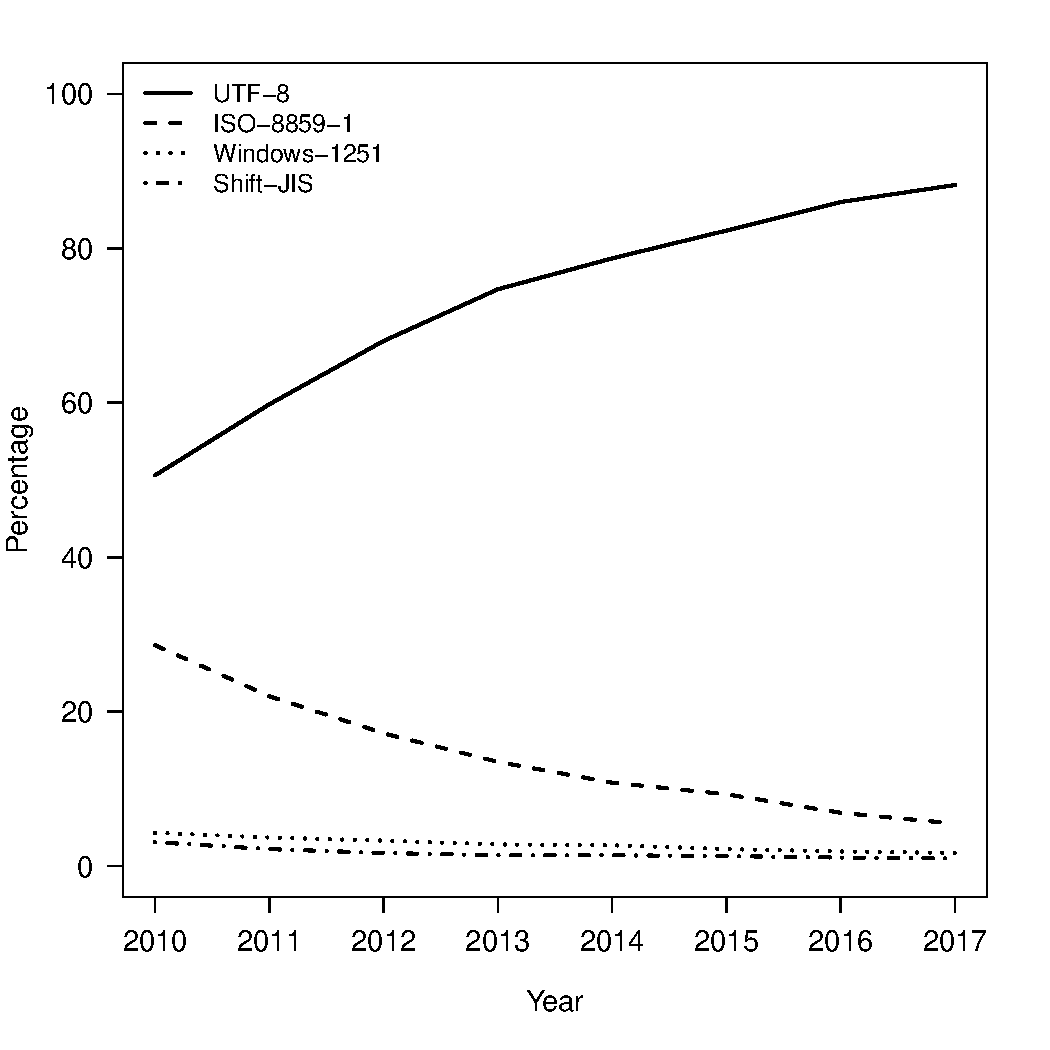
\includegraphics[width=0.7\textwidth]{fig/encoding_use.pdf}
\caption{Percentages of encoding standards used on the web \citep{w3techs2017}.}
\label{fig:encoding}
\end{figure}

The different data types within a file are to be formatted according to
commonly used standards where possible. In particular, data in validation
reports are encoded as stated in Table~\ref{tab:dataformat}.
\begin{center}
\captionof{table}{Format of data types in validation reports.}
\begin{tabular}{|lp{0.92\textwidth}|}
\hline
1&Numbers are encoded in a valid decimal ISO/IEC/IEEE 60559:2011 (IEEE 754) format
\citep{ieee:2008}. \\
2&Date-time data shall be denoted in ISO 8601 format \code{YYMMDDTHHmmss+HHMM} \citep{iso2004data}. \\
\hline
\end{tabular}
\label{tab:dataformat}
\end{center}

%%%%%%%%%%%%%%%%%%%%%%%%%%%%%%%%%%%%%%%%%%%%%%%%%%%%%%%%%%%%%%%%%%%%%%%%%%%%%%%
\clearpage{}
\subsection{JSON messages}
\label{sect:jsonmessage}


\begin{align*}
\langle \textsf{key}, \textsf{type}, 
\textsf{event}, \textsf{expression}, \textsf{data}, \textsf{value}\rangle
\end{align*}





\clearpage{}
%%%%%%%%%%%%%%%%%%%%%%%%%%%%%%%%%%%%%%%%%%%%%%%%%%%%%%%%%%%%%%%%%%%%%%%%%%%%%%%
\subsection{JSON Schemas}
In this subsection the JSON schemas defining the basic and extended
validation reports and their components are listed as a reference.

The full code can also be found at github:
\begin{center}
\href{https://github.com/data-cleaning/ValidatReport}{https://github.com/data-cleaning/ValidatReport}
\end{center}
%
\lstinputlisting[frame=single
  , linewidth=1.1\textwidth
  , float=h,caption=JSON schema for a confrontation object.
  , label=lst:confrontation]{../json/validation_report.json}
%
%



